%! TEX root = thesis.tex

\chapter{Results}
\label{sec:results}

\section{Pareto Frontier Analysis}
\label{sec:pareto}

Figure~\ref{fig:pareto} presents the combined Pareto frontiers for both models
across all five regions.  Table~\ref{tab:best} reports the best-score
configurations with optimized start dates.

\begin{figure}
  \centering
  
\includegraphics[width=0.75\textwidth]{figures/savings_vs_overhead_all}
  \caption{Combined Pareto frontiers for DeepSeek~V3 and Kimi~K2 across five
  grid regions.  Each point is a feasible policy evaluated on 2025 5-minute
  intensity data.  Best-score points within 200\% overhead are highlighted.}
  \label{fig:pareto}
\end{figure}

For DeepSeek~V3, single-year savings range from 43.4\% (Germany, score 0.717)
to 6.2\% (China, score 0.531).  High-variability grids (Germany, Italy)
extend to high overheads (approaching 200\%) with correspondingly high
savings, while low-variance grids (US, CN) exhibit compressed frontiers
regardless of policy choice.

In high-variability grids, the frontier reflects abundant dirty intervals
worth avoiding.  Sweden plateaus earlier because the grid is so clean on
average that fewer dirty intervals exist.  The US and China show limited
temporal variation: pausing rarely finds a significantly cleaner interval than
the one it left.

For Kimi~K2, the same regional ordering holds at lower absolute savings
(Germany 27.5\%, score 0.637; China 2.4\%, score 0.512).  Larger GPU counts
amplify the benefit of avoiding dirty intervals, but the scaling is
sub-linear: DeepSeek~V3's up to 8$\times$ GPU advantage yields only 1.5 to
2.0$\times$ the relative savings, because checkpoint overhead also scales with
GPU count.

    \begin{table}
    \centering
    \caption{Best policy configurations per (model, region) with optimized
    start dates.  The hysteresis margin $\Delta_\theta = \theta_p - \theta_r$
    is at most 16~gCO$_2$eq/kWh across all combinations.}
    \label{tab:best}
    \small
    \begin{tabular}{llrrrrr}
      \toprule
      Model & Region & $\theta_p$ & $\theta_r$ & Savings & Overhead & Score \\
      \midrule
      DeepSeek~V3 & DE & 272 & 268 & 43.4\% & 174.3\% & 0.717 \\
      DeepSeek~V3 & IT & 246 & 231 & 32.7\% & 194.7\% & 0.663 \\
      DeepSeek~V3 & SE &  19 &  18 & 23.2\% & 106.3\% & 0.616 \\
      DeepSeek~V3 & US & 396 & 386 &  9.5\% & 115.7\% & 0.547 \\
      DeepSeek~V3 & CN & 528 & 512 &  6.2\% &  72.5\% & 0.531 \\
      \midrule
      Kimi~K2 & DE & 267 & 262 & 27.5\% & 199.4\% & 0.637 \\
      Kimi~K2 & IT & 283 & 271 & 16.6\% & 129.1\% & 0.583 \\
      Kimi~K2 & SE &  22 &  21 & 12.8\% & 115.4\% & 0.564 \\
      Kimi~K2 & US & 453 & 447 &  3.1\% &  22.2\% & 0.516 \\
      Kimi~K2 & CN & 537 & 522 &  2.4\% &  40.1\% & 0.512 \\
      \bottomrule
    \end{tabular}
\end{table}

The ranking of regions by savings potential (DE > IT > SE > US > CN) follows
the ranking by coefficient of variation.  Mean intensity plays a
secondary role: Sweden's high coefficient of variation is offset by its very low mean (23
gCO$_2$eq/kWh), limiting the absolute emissions available to avoid.

\section{Threshold Space and Hysteresis Margin}
\label{sec:threshold-space}

The central finding of this work emerges from the threshold space analysis.
Figure~\ref{fig:threshold} shows the pause vs.\ resume threshold plane for
DeepSeek~V3 in Germany, with color encoding the composite score.

\begin{figure}
  \centering
  
\includegraphics[width=0.75\textwidth]{figures/threshold_space_DeepSeek_V3_DE_0101}
  \caption{Pause vs.\ resume threshold for DeepSeek~V3 in Germany.  Color
  encodes composite score.  The diagonal $\theta_r = \theta_p$ marks
  zero-hysteresis policies.  High-scoring configurations cluster within a
  narrow margin, demonstrating that wide hysteresis margins are never
  Pareto-optimal.}
  \label{fig:threshold}
\end{figure}

Optimal hysteresis margins cluster near zero.  Across all 10 (model, region)
combinations, the best-score points satisfy the condition $\Delta_\theta \leq
16$~gCO$_2$eq/kWh, and in most cases $\Delta_\theta \leq
10$~gCO$_2$eq/kWh.  Zero-hysteresis policies ($\theta_r = \theta_p$) achieve
scores within 1--3\% of the optimum, confirming that a non-zero margin
provides marginal practical benefit.

Figure~\ref{fig:margin} confirms this pattern across the full policy set for
Kimi~K2.  Beyond $\Delta_\theta \approx 50$~gCO$_2$eq/kWh, wider margins
accumulate idle time and checkpoint overhead without proportional additional
savings.  A wide margin means training resumes only at very low intensities,
remaining paused through moderately clean intervals that could have been
exploited.

\begin{figure}
  \centering
  
\includegraphics[width=\textwidth]{figures/margin_vs_best_Kimi_K2}
  \caption{Composite score vs.\ hysteresis margin $\Delta_\theta$ for
  Kimi~K2.  Scores peak at $\Delta_\theta < 16$~gCO$_2$eq/kWh and plateau
  beyond $\Delta_\theta \approx 50$~gCO$_2$eq/kWh.  Zero-margin policies
  score within 1--3\% of the optimum.}
  \label{fig:margin}
\end{figure}

This finding is robust across two models and five regions, suggesting that a
near-zero margin is a fundamental property of the problem rather than an
artifact of our experimental settings.

\section{Start Date Sensitivity}
\label{sec:start-date}

Start date exerts a measurable but secondary influence on policy performance.
Across all (model, region) combinations, winter months (November to February)
are disproportionately represented among optimal start dates.  This reflects
lower grid carbon intensity during the heating season in many regions.

The effect ranges from approximately 20 percentage points of savings (Italy) to
under 2 percentage points (China), confirming that the hysteresis threshold
choice mostly, but not always, dominates start-date scheduling.

\section{Threshold Generalization Across Years}
\label{sec:threshold-generalization}

The best-scoring hysteresis threshold pairs for each model are not consistent across years.
Figure~\ref{fig:threshold-generalization} shows that the best-scoring thresholds for each model vary from year
to year, indicating that the optimal thresholds are sensitive to the specific carbon intensity
patterns of each year.  This suggests that a static threshold policy may not be optimal across
different years, and adaptive or year-specific threshold tuning could yield better performance
in terms of emissions savings and overhead management.

\begin{figure}
  \centering
  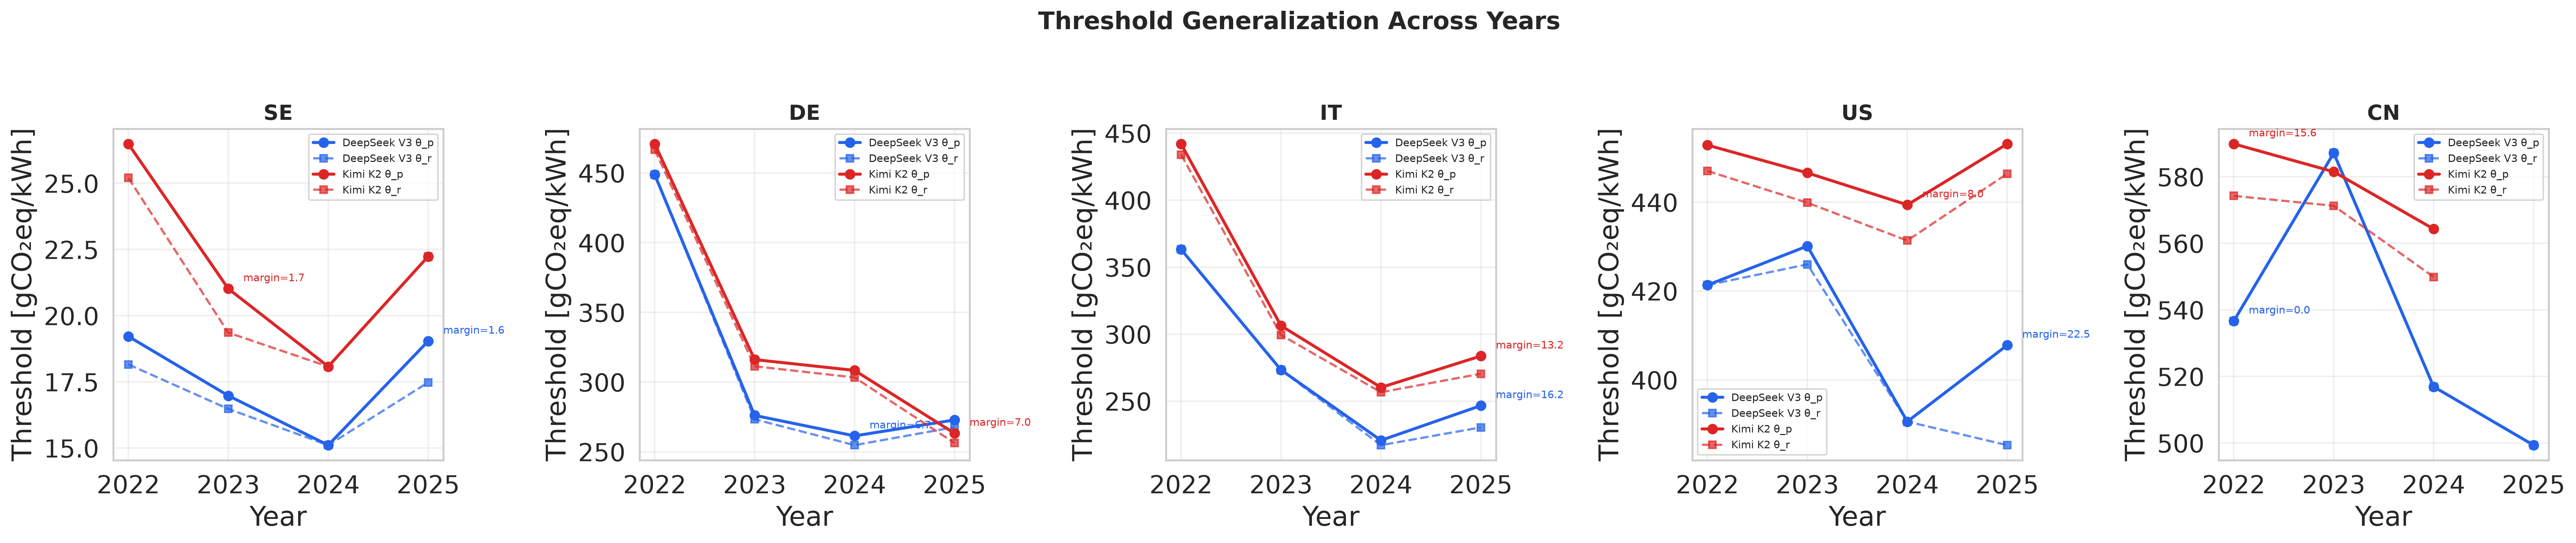
\includegraphics[width=1\textwidth]{figures/threshold_generalization}
  \caption{Threshold Generalization: Best scoring hysteresis threshold pairs for each model across the years from 2022 to 2025.}
  \label{fig:threshold-generalization}
\end{figure}


\section{Optimizer Convergence}
\label{sec:convergence}

The adaptive grid-search optimizer converges rapidly.  Figure~\ref{fig:convergence}
shows the score improvement across iterations for all (model, region)
combinations.  The score improves substantially between iterations 1 and 5,
plateaus by iteration 5 or 6, and subsequent iterations provide only marginal
refinement.

\begin{figure}
  \centering
  
\includegraphics[width=0.75\textwidth]{figures/score_vs_iteration_all}
  \caption{Optimizer convergence: composite score vs.\ iteration number for
  all (model, region) combinations.  Score plateaus by iteration 5--6 in all
  cases.}
  \label{fig:convergence}
\end{figure}
